\documentclass[a4paper, 12pt, twoside]{article}

\usepackage[francais]{babel}
\usepackage[utf8]{inputenc}
\usepackage{lmodern}
\usepackage[T1]{fontenc}
\usepackage{layout}

\usepackage{fancyhdr}
\usepackage{soul}
\usepackage{url}
\usepackage{color}
\usepackage{graphicx}
\usepackage{array}
\usepackage{geometry}

\title{\hrule \vspace{1cm} Cachier des charges : PicExplorer}
\author{\textsc{Lanvin} Elyan - \textsc{Marcais} Thomas\\ \textsc{Ramolet} Arthur - \textsc{Guenver} Loïc\\ \textsc{Aydin} Emre - \textsc{Foucault} Antoine}
\date{\today}

\begin{document}

%Définition du style des bords de page
\pagestyle{fancy}
\lhead{}
\chead{}
\rhead{\leftmark}
\lfoot{Groupe C}
\cfoot{}
\rfoot{Page \thepage}

%Titre
\clearpage\thispagestyle{empty}

\maketitle
\begin{center}
 \copyright 2014 Groupe C - Tout droit reservé\\
\end{center}
\vspace{1cm}
\hrule

\newpage

%Sommaire
\renewcommand{\contentsname}{Sommaire}
\tableofcontents
\newpage

%Corps
\section{Présentation du projet}

\subsection{Contexte}

Ce projet se déroulera dans le cadre d'un projet tutoré lors du semestre 6 de L3 SPI Informatique. Ce document définit les exigences et les besoins du client, ainsi que les fonctionnalités qui seront présentes dans la future application.

\subsection{Étude de l'existant}

\begin{description}

  \item[Hanjie-star :] Jeu de picross en ligne gratuit\footnote{Disponible sur le lien suivant : \url{www.hanjie-star.fr}}
  \item[Picross Nintendo\copyright :]  Jeu de picross sur Nintendo\copyright \space DS
  \item[Zelda Picross :] Jeu de picross amateur open source

\end{description}

La partie ci-dessous décrit les différentes fonctions communes et spécifiques des trois applications : \newline

\begin{itemize}\setlength{\itemsep}{5mm}

  \item[\textbullet] \large\textbf{Fonctions communes\newline}
  
  \begin{itemize}\setlength{\itemsep}{2mm}
  \item Cocher case valide
  \item Cocher case non valide
  \item Cocher en continu (en faisant glisser la souris)
  \item Timer
  \item Vérifier la grille
 \end{itemize}

 \item[\textbullet] \large\textbf{Hanjie-star\newline}
 
 \begin{itemize}\setlength{\itemsep}{2mm}
  \item Éditeur
  \item Recherche de grille dans la base (sur différents critères de description de grilles)\newline
 \end{itemize}

 \item[\textbullet] \large\textbf{Picross Nintendo\copyright\newline}
 
 \begin{itemize}\setlength{\itemsep}{2mm}
  \item Correction temps réel (pénalité de temps et signalement en cas d'erreur)
  \item Pas de remplacement
  \item Tactile
 \end{itemize}
 
 \item[\textbullet] \large\textbf{Zelda Picross\newline}
 
 \begin{itemize}\setlength{\itemsep}{2mm}
  \item Mode aventure
 \end{itemize}
 
\end{itemize}

\subsection{Objectifs}

Ce projet doit aboutir à la création d'une application de type jeu de picross (ou henjie), destinée à tout public. Un système d'aide permettra de terminer une grille, peu importe son expérience et la difficulté de la grille.\newline

L'application comprendra :\newline

\begin{itemize}\setlength{\itemsep}{3mm}
 \item La résolution d'une grille de picross
 \item Un éditeur pour créer ses propres grilles
 \item Un système d'aide à la résolution
 \item Un système de sauvegarde/chargement (persistance des données)
 \item Un tutoriel (sous forme de pop-up/fenêtre d'aide)
\end{itemize}

\subsection{Calendrier}

La soutenance est prévue pour le vendredi 16 mai à 13h30, le projet est à rendre la semaine précédente au plus tard.
Le premier cycle de programmation devrait se terminer le 14/03/2014.

\subsection{Critères d'acceptibilité du produit}

L’application doit répondre aux critères suivants :\newline

\begin{itemize}

 \item Validation du produit via un dossier de tests réalisé par notre groupe
 \item Respect des contraintes client (choix technologique, fonctionnalités de l'application)
 
\end{itemize}

\section{Analyse des besoins}

\subsection{Liste des acteurs}

\ul{L'utilisateur :}\newline

À l'aide de l'application, l'utilisateur pourra éditer ses propres grilles de Picross en noircissant les cases de la grille comme voulu. \\Il peut également générer un fichier de sauvegarde de sa grille qui sera exportable avec d'autres applications.
L'utilisateur pourra également se servir de l'application pour jouer au Picross. Il pourra sélectionner une des grilles à résoudre par défaut ou il pourra importer des grilles éditées au préalable.\\ Lors de la résolution des grilles, il pourra faire appel à une aide de la machine. Il peut également consulter les statistiques et classements du jeu.

\subsection{Expression des besoins}

Le client souhaite disposer d'une application réalisée sous Ruby. Celle-ci sera décomposée en deux grandes parties :\newline

\begin{itemize}\setlength{\itemsep}{3mm}

  \item[\textbullet] L'édition de grilles de Picross via une interface simple permettant de noircir la grille voulue ou de générer une grille aléatoirement.\newline
  \item[\textbullet] La résolution des grilles de Picross, selon les règles traditionnelles du jeu, avec possibilité de demander de l'aide au jeu si le joueur est bloqué.
 'application doit également être capable de charger, au démarrage, la dernière grille en cours.

\end{itemize}
 
\subsection{Besoins fonctionnels}

\ul{\'Edition des grilles de Picross :}\newline

\begin{itemize}\setlength{\itemsep}{5mm}

 \item[\textbullet] Création d'une nouvelle grille de Picross à partir d'une grille vierge\newline
 \begin{itemize}
  \item L'utilisateur devra choisir la taille de grille puis noircir les cases tel qu'il le souhaite
 \end{itemize}

 \item[\textbullet] Création d'une grille de Picross aléatoirement\newline
 \begin{itemize}
  \item L'utilisateur doit avoir la possibilité, via un bouton par exemple, de noircir aléatoirement une grille dans l'éditeur. Il lui est également possible de la modifier manuellement par la suite
 \end{itemize}

 \item[\textbullet] Exportation d'une grille\newline
 \begin{itemize}
  \item Après avoir édité sa grille, l'utilisateur peut générer un fichier de sauvegarde de sa grille qu'il pourra partager avec d'autres utilisateurs
 \end{itemize}

 \item[\textbullet] Modification d'une grille existante\newline
 \begin{itemize}
  \item L'utilisateur peut modifier une grille qu'il a créé préalablement
 \end{itemize}

\end{itemize}

\ul{R\'esolution des grilles de Picross :}\newline

\begin{itemize}\setlength{\itemsep}{5mm}

 \item[\textbullet] Démarrer une partie\newline
 \begin{itemize}
  \item L'utilisateur doit choisir entre deux modes : \og Grilles par défaut \fg ou \og Grilles importées \fg. Ensuite il sélectionne la grille à laquelle il souhaite jouer
 \end{itemize}

 \item[\textbullet] Aide à la résolution automatique\newline
 \begin{itemize}
  \item Lors d'une partie, le joueur peut demander l'aide du jeu s'il se voit bloqué. Différents niveaux d'aide sont disponibles : résolution d'une case ou conseils
 \end{itemize}
 
 \item[\textbullet] Sauvegarder la grille en cours\newline
 \begin{itemize}
  \item L'application doit pouvoir gérer différentes manières de sauvegarder ses parties en cours. Soit l'application garde la dernière partie en cours en mémoire et propose de la reprendre au démarrage, soit on peut sauvegarder la partie en cours via une option dans la barre de menu
 \end{itemize}
 
 \item[\textbullet] Importation d'une grille\newline
 \begin{itemize}
  \item L'utilisateur doit pouvoir importer une grille sous forme de fichier de sauvegarde pour pouvoir y jouer
 \end{itemize}
 
\end{itemize}

\subsection{Besoins non-fonctionnels}

\begin{itemize}\setlength{\itemsep}{3mm}

 \item[\textbullet] Sérialisation des objets pour persistance\newline
 \begin{itemize}
  \item L'application a la possibilité, à son extinction,  de sérialiser les grilles, les statistiques et les options afin de pouvoir les récupérer au redémarrage de l'application
 \end{itemize}
 
\end{itemize}

\subsection{Fonctionnalités}%Remplir les tableaux et spécifications

\subsubsection*{Le jeu}

\begin{center}

  \begin{tabular}{|>{\centering\arraybackslash}m{0.2\linewidth}|>{\centering\arraybackslash}m{0.7\linewidth}|}
  \hline
  \textbf{R\'ef\'erence} & \textbf{Fonctionnalit\'e} \\
  \hline
  & \textcolor{blue}{Traitement/Persistance des donn\'ees} \\[5ex]
  \hline
  3 & Sauvegarder/Charger les options\\
  \hline
  3 & Sauvegarder/Charger une partie\\
  \hline
  3 & Sauvegarder/Charger les scores et les statistiques\\
  \hline
  3 & Crypter les données [OPTION]\\
  \hline
  & \textcolor{blue}{Jeu}\\[5ex]
  \hline
  3 & Jouer une partie\\
  \hline
  3 & Système d'aide\\
  \hline
  \end{tabular}

\end{center}

\begin{itemize}
 \item[\textbullet] \textbf{\textcolor{blue}{Jeu : }}
 \begin{description}
    \item[Aider le joueur :]  L'utilisateur doit pouvoir recevoir une aide du logiciel dans le cas ou il est bloqué. Il pourra interagir sur le  plateau de deux différentes manières. Noircir une case correcte ou donner un indice à l'utilisateur
     \item[Jouer une partie :] L'utilisateur doit pouvoir jouer une partie de Picross à l'aide de la souris
  \end{description}
  
  \item[\textbullet] \textbf{\textcolor{blue}{Traitement et persistance des données : }}
 \begin{description}
    \item[Sauvegarder/Charger les options :] Les choix de l'utilisateur concernant les options du jeu sont sauvegardées entre les différents lancements du jeu
    \item[Sauvegarder/Charger une partie :] L'utilisateur peut sauvegarder sa partie en cours afin de la reprendre ultérieurement.\\Lorsqu'il quitte le jeu en pleine partie et qu'il revient, le jeu lui propose de reprendre la partie précédente ou de retomber sur les menus
    \item[Sauvegarder/Charger les scores et les statistiques :]
    \item[Crypter les données [OPTION] :] Toute donnée sauvegardée sur le système est cryptée de façon à assurer l'intégrité des sauvegardes
  \end{description}
\end{itemize}

\subsubsection*{L'éditeur}

\begin{center}

  \begin{tabular}{|>{\centering\arraybackslash}m{0.2\linewidth}|>{\centering\arraybackslash}m{0.7\linewidth}|}
  \hline
  \textbf{Référence} & \textbf{Fonctionnalité} \\
  \hline
  & \textcolor{blue}{Traitement/Persistance des donn\'ees} \\[5ex]
  \hline
  3 & Sauvegarder/Charger un plateau \\
  \hline
  & \textcolor{blue}{\'Editeur}\\[5ex]
  \hline
  3 & Créer un plateau aléatoirement \\
  \hline
  3 & Créer une grille \\
  \hline
  3 & Modifier une grille \\
  \hline
  \end{tabular}
 
\end{center}

\begin{itemize}
 \item[\textbullet] \textbf{\textcolor{blue}{\'Editeur : }}
 \begin{description}
    \item[Créer une grille :] L'utilisateur doit pouvoir créer une grille personnalisé en remplissant une grille vide
    \item[Créer une grille aléatoirement :] L'application doit pouvoir créer une grille aléatoire pour l'utilisateur
    \item[Modifier une grille :] L'utilisateur doit pouvoir modifier une grille déjà existante
  \end{description}
  
  \item[\textbullet] \textbf{\textcolor{blue}{Traitement et persistance des données : }}
 \begin{description}
    \item[Sauvegarder/Charger un plateau :] L'utilisateur doit pouvoir sauvegarder ses plateaux en cours et si l'application quitte sans avoir sauvegarder, le dernier plateau est sauvegarder automatiquement
  \end{description}
\end{itemize}

\begin{figure}[ht]
  \center
  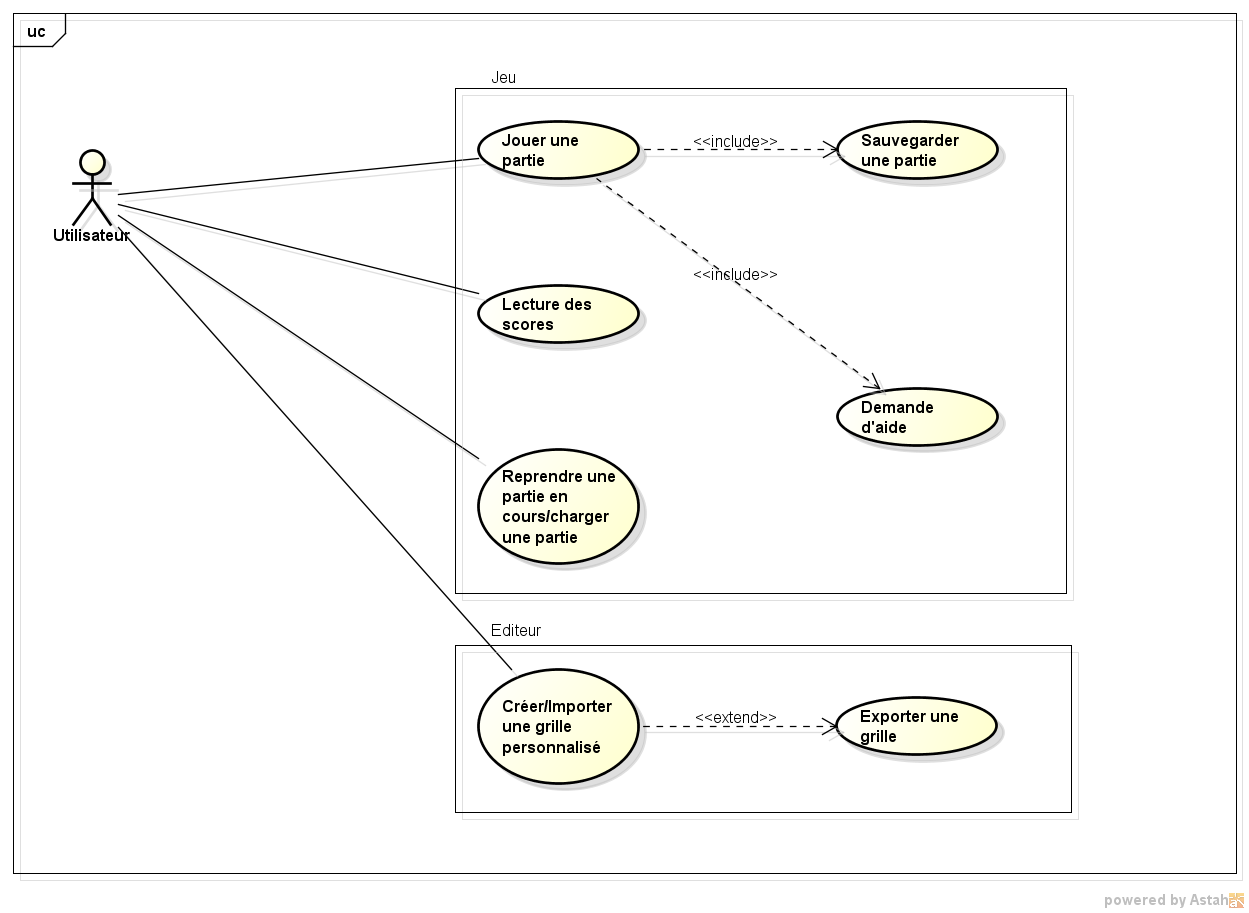
\includegraphics[scale=0.50]{CasUt.png}
  \caption{Diagramme de cas d'utilisation}
  \label{diagCU}
\end{figure}

\subsection{Cas d'utilisation} % Finir de remplir les différents cas d'utilisation

\subsubsection*{Cas d'utilisation \no1}

\begin{description}\setlength{\itemsep}{0mm}

 \item[Nom :] Résolution picross  
 \item[Description :] L’utilisateur tente de résoudre une grille de picross 
 \item[Acteur :] L'utilisateur de l'application 
 \item[Préalables :]  L'application doit être téléchargée
 \item[Conséquents :] L'utilisateur peut exécuter l'application\newline
 
\end{description}

\begin{enumerate}
	\item{\ul{Choix des options :}}\newline
	\begin{itemize}\setlength{\itemsep}{5mm}
		\item L’utilisateur clique sur l'option "nouvelle partie".\newline
		\item Le système demande si l'on souhaite une grille choisie ou aléatoire.
		\item {Si l'utilisateur demande une grille al\'eatoire :}
		\begin{itemize}
			\item Le système propose différentes tailles de grille (Peut être encombrant s'il y en a beaucoup, mais évite une entrée manuelle qui pourrait être incorrecte).\newline
		\end{itemize}	

		\item L'utilisateur choisit une taille.
		\item Le système s\'electionne une grille.
		\item Ajout d'un malus par joker utilis\'e.
		\item {Dans le cas ou le nombre au départ est limit\'e :}
		\begin{itemize}\setlength{\itemsep}{3mm}
			\item Ajout d'un bonus en fonction du nombre de jokers non utilisés (optionnel).\newline
		\end{itemize}	
		\item On considère que le timer est toujours mis en place.
		\end{itemize}

	\item{\ul{R\'esolution du picross :}}\newline
	\begin{itemize}\setlength{\itemsep}{5mm}
		\item L'utilisateur essaye de résoudre la grille.
		\item L'utilisateur peut utiliser l'option "joker / aide" pour se débloquer.
		\item Une fois la grille complète, il peut cliquer sur l'option "terminer / vérifier grille"\newline

		\item Le système compare les valeurs de chaque ligne / colonne avec les cases noircies.
		\item Affichage d'un message indiquant s'il y a correspondance (réussite) ou non.\newline

		\item {S'il y a correspondance :}
		\begin{itemize}\setlength{\itemsep}{3mm}
			\item Enregistrement du temps mis pour terminer la grille, suivant le profil.
			\item Affichage des records pour cette grille.
			\item {Si l\'image obtenue est diff\'erente de celle stock\'ee :}
			\begin{itemize}\setlength{\itemsep}{1mm}
				\item Le système en informe l'utilisateur et lui montre l'image en question.\newline
			\end{itemize}					
		\end{itemize}	
		\item Le système propose soit de tenter une nouvelle grille, soit de retourner au menu principal.
		\item L'utilisateur choisit.\newline

		\item {Sinon :}
		\begin{itemize}\setlength{\itemsep}{3mm}
			\item L'utilisation d'un joker peut être proposé dans le message, puisque le joueur s'en servira probablement pour repérer une erreur.
		\end{itemize}			
	\end{itemize}

	\item{\ul{Exceptions :}}\newline
	\begin{itemize}\setlength{\itemsep}{5mm}
		\item L'utilisateur entre une taille de grille souhaitée qui n'est pas prise en compte (dans le cas d'une saisie manuelle).
		\item L'utilisateur veut utiliser un joker alors qu'il n'en a plus.
	\end{itemize}
\end{enumerate}

\subsubsection*{Cas d'utilisation \no2}

\begin{description}\setlength{\itemsep}{0mm}

 \item[Nom :] \'Edition picross 
 \item[Description :] L'utilisateur créé une grille de picross via l'éditeur
 \item[Acteur :] L'utilisateur de l'application 
 \item[Préalables :] L'application doit être téléchargée
 \item[Conséquents :] L'utilisateur peut exécuter l'application\newline
 
\end{description}

\begin{enumerate}
	\item{\ul{Cr\'eation de la grille :}}\newline
	\begin{itemize}	\setlength{\itemsep}{5mm}
		\item L'utilisateur clique sur l'option "créer un picross".
		\item Le système permet de modifier le nombre de lignes et de colonne soit avec une saisie manuelle.
		\item Un "pointeur" situé sur une barre de longueur 25.\newline

		\item L'utilisateur sélectionne le nombre de lignes et de colonnes (non modifiable par la suite).
		\item L'utilisateur dessine son image en cliquant sur les cases de la grille pour les noircir, une 2e fois pour annuler.
		\item L'utilisateur clique sur l'option "enregistrer la grille".
	\end{itemize}
	\item{\ul{Enregistrement de la grille :}}\newline
	\begin{itemize}	\setlength{\itemsep}{5mm}
		\item Le système demande de saisir un nom de grille (obligatoire) ainsi qu'une description (optionnel, peut aider à résoudre la grille).
		\item L'utilisateur saisit le nom, et éventuellement la description.
		\item Le système compte, pour chaque ligne et ensuite pour chaque colonne, les séries de cases noires et enregistre ces valeurs avec la grille.\newline

		\item Le système propose soit de créer une autre grille, soit de retourner au menu principal.
		\item L'utilisateur choisit.
	\end{itemize}


\end{enumerate}

\section{Livrables}

\begin{itemize}\setlength{\itemsep}{3mm}

 \item[\textbullet] Un cahier des charges validé par le client
 \item[\textbullet] Un logiciel qui respecte le cahier des charges
 \item[\textbullet] Les cahiers d'analyse et de conception
 \item[\textbullet] Un manuel utilisateur
 
\end{itemize}

\section{Contraintes}

\subsection{Documentation}

\begin{tabular}{|>{\centering\arraybackslash}m{0.4\linewidth}|>{\centering\arraybackslash}m{0.6\linewidth}|}
  \hline
  \textbf{Document} & \textbf{Objectif}\\
  \hline
  Cahier des charges & Spécifier les besoins du client, les fonctionnalités attendues de l'application, ainsi que les contraintes liées au projet\\
  \hline
  Dossier d'analyse et de conception & Présenter les outils et technologies utilisées dans le cadre du projet et préciser son architecture\\
  \hline
  Manuel utilisateur & Indiquer à l'utilisateur comment utiliser les différentes fonctionnalités présentes dans l'application\\
  \hline
\end{tabular}


\subsection{Délais}%Ajouter date de rendu du CDC

Tous les livrables qui accompagnent l'application, ainsi que l'application elle-même doivent être rendus le ????.

\subsection{Contraintes techniques}

Le développement de l'application se fera avec ces moyens techniques listés ci-dessous :\newline

\begin{itemize}\setlength{\itemsep}{3mm}

 \item[\textbullet] Compatibilité avec le langage Ruby dans sa version 1.9.3 et inférieur
 \item[\textbullet] Interface graphique avec la bibliothèque logicielle GTK
 \item[\textbullet] Mise en \oe uvre de la persistance des données à l'aide de la sérialisation
 \item[\textbullet] Environnement technique (système d’exploitation, langage de programmation ...)
 
\end{itemize}

\section{Organisation du projet}


%Ajout du diagramme WBS dans une page dédiée
\newpage\thispagestyle{empty}
\newgeometry{top=0.5cm, bottom=0cm, left=0.5cm, right=0.5cm}

\subsection{Diagramme WBS}

\begin{figure}[!h]
  \center
  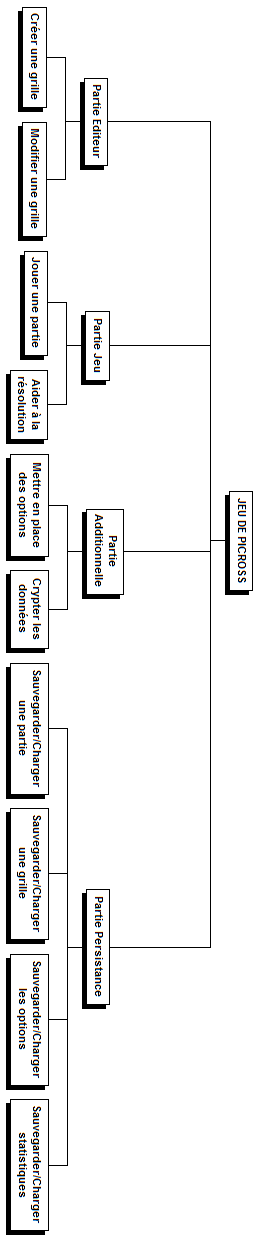
\includegraphics[scale=0.61]{WBS.png}
  \caption{Diagramme WBS du projet}
  \label{diagWBS}
\end{figure}

\newpage
\restoregeometry

%Fin WBS

\subsection{Diagramme de Gantt}

\end{document}
